%% This is the main file and you use this file to organize your assignment.

\documentclass[a4paper]{article}
\usepackage[margin=3cm]{geometry} 	   % Choose your margin here.
\usepackage{amsmath}
\usepackage{gensymb}
\usepackage{amssymb}
\usepackage{parskip}
\usepackage{graphicx}
\usepackage{caption}
\usepackage{subcaption}
\usepackage{color} %red, green, blue, yellow, cyan, magenta, black, white
\definecolor{mygreen}{RGB}{28,172,0} % color values Red, Green, Blue
\definecolor{mylilas}{RGB}{170,55,241}
\usepackage{float}
\usepackage{listings}

\renewcommand\thesection{Problem \arabic{section}}
\renewcommand\thesubsection{\alph{subsection})}

\newcommand{\figref}[1]{\figurename~\ref{#1}}

\let\endtitlepage\relax						% Begin the text immidiately after the title page. Optional
\setlength{\parindent}{0cm}				% Start paragraph without indent. Optional

\begin{document}

\lstset{language=Matlab,%
    breaklines=true,%
    morekeywords={matlab2tikz},
    keywordstyle=\color{blue},%
    morekeywords=[2]{1}, keywordstyle=[2]{\color{black}},
    identifierstyle=\color{black},%
    stringstyle=\color{mylilas},
    commentstyle=\color{mygreen},%
    showstringspaces=false,%without this there will be a symbol in the places where there is a space
    numbers=left,%
    numberstyle={\tiny \color{black}},% size of the numbers
    numbersep=9pt, % this defines how far the numbers are from the text
    emph=[1]{for, end, break}\emphstyle=[1]\color{red}, %some words to emphasise
}

\begin{titlepage}
\begin{center}
\Large TTK4190 Guidance and Control of Vehicles \\
\vspace{10pt}
Assignment 2 \\
\vspace{10pt}
\large Written Fall 2019 By Martin Gerhardsen and Sigurd Totland
\end{center}
\end{titlepage}

\section{Open loop analysis}

\subsection{}
Since the wind speed $\mathbf{V}_w$ is assumed zero, we have that the ground speed is
\begin{equation}\begin{aligned}
\label{eq:ground_air}
\mathbf{V}_g = \mathbf{V}_a - \mathbf{V}_w = \mathbf{V}_a.
\end{aligned}\end{equation}

\subsection{}
The definition of crab angle from REF:BEARD is
\begin{equation}\begin{aligned}
\chi_c \triangleq \chi - \psi
\end{aligned}\end{equation}
where $\chi$ is the course and $\psi$ is the heading. Since the wind speed is assumed zero, the sideslip $\beta = \chi_c$ and so
\begin{equation}\begin{aligned}
\beta = \chi - \psi.
\end{aligned}\end{equation}
We can also express this using the velocity of the aircraft. From equation (2.8) in REF:BEARD, we have that
\begin{equation}\begin{aligned}
\beta = \sin^{-1}\left(\frac{v_r}{\sqrt{u^2_r + v^2_r + w^2_r}}\right) = \sin^{-1}\left(\frac{v_r}{V_a}\right),
\end{aligned}\end{equation}
or since $\mathbf{V}_g = \mathbf{V}_a$,
\begin{equation}\begin{aligned}
\beta = \sin^{-1}\left(\frac{v_r}{V_g}\right).
\end{aligned}\end{equation}

\subsection{}
From REF:BEARD, we have that the characteristic function of the dutch-roll mode is
\begin{equation}\begin{aligned}
s^2 + (-Y_v - N_r)s + (Y_vN_r - N_vY_r) = 0.
\end{aligned}\end{equation}
With that, we have that the natural frequency $\omega_0$ and relative damping ratio $\zeta$, as in
\begin{equation}\begin{aligned}
s^2 + 2\zeta \omega_0 s + \omega_0^2 = 0,
\end{aligned}\end{equation}
are respectively
\begin{equation}\begin{aligned}
\omega_0 = \sqrt{Y_v N_r - N_v Y_r} \quad \text{and} \quad \zeta = -2\frac{Y_v + N_r}{\omega_0}.
\end{aligned}\end{equation}

\subsection{}
\begin{figure}[ht]
	\centering
	\begin{subfigure}[b]{0.45\textwidth}
		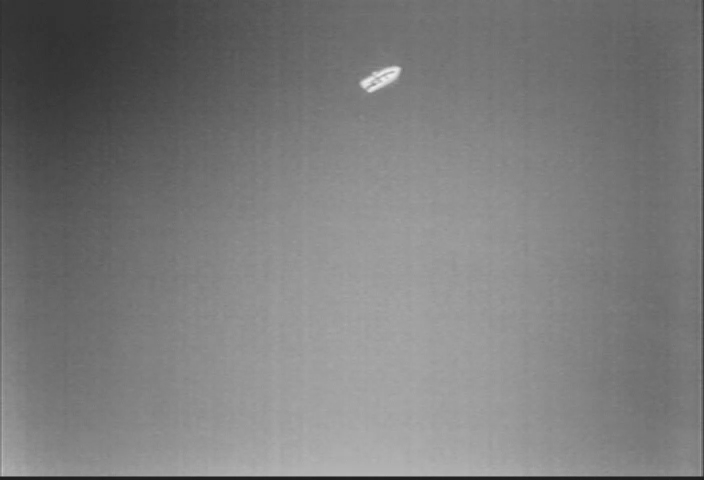
\includegraphics[width=\textwidth]{fig1}
		\caption{caption..}
		\label{fig:2a}
	\end{subfigure}
	~ %add desired spacing between images, e. g. ~, \quad, \qquad, \hfill etc.
	%(or a blank line to force the subfigure onto a new line)
	\begin{subfigure}[b]{0.45\textwidth}
		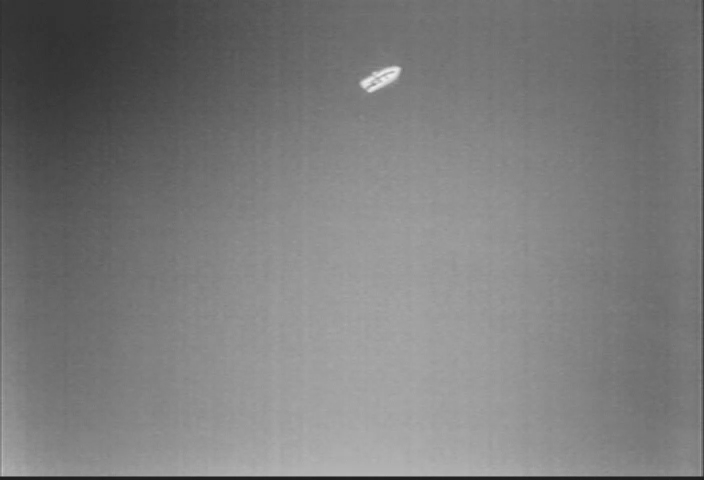
\includegraphics[width=\textwidth]{fig1}
		\caption{caption..}
		\label{fig:2b}
	\end{subfigure}
	\begin{subfigure}[b]{0.45\textwidth}
		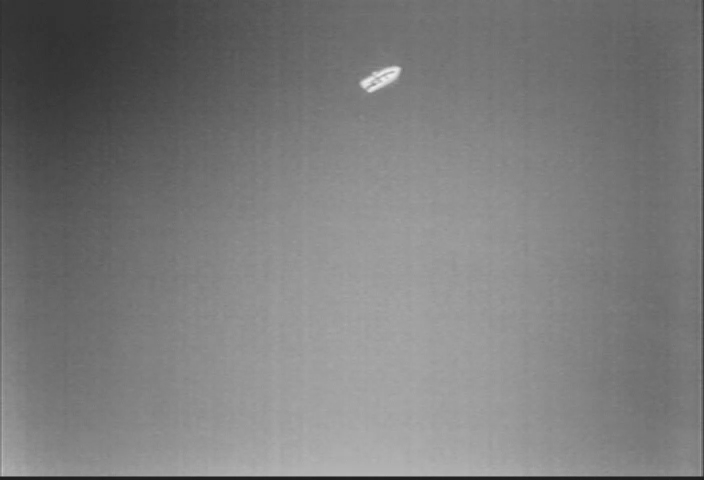
\includegraphics[width=\textwidth]{fig1}
		\caption{caption..}
		\label{fig:2c}
	\end{subfigure}
	\begin{subfigure}[b]{0.45\textwidth}
		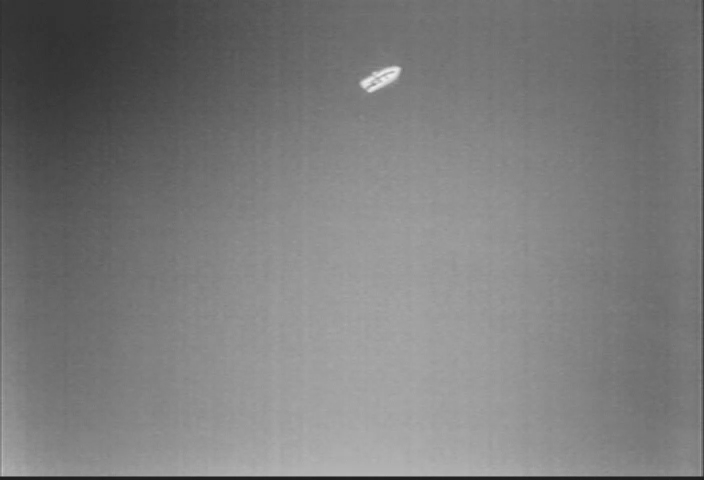
\includegraphics[width=\textwidth]{fig1}
		\caption{caption..}
		\label{fig:2d}
	\end{subfigure}
	\caption{Caption for all figures}\label{fig:2}
\end{figure}
	% Use "\include" instead of "\input" if you want the section to start on a new page. "problem1" is a tex file included at this location in the document. It is possible to answer the whole assignment in the main file (paste everything from "problem1.tex" and "problem2.tex" here), but that restricts the readability. Therefore, one file is created for each problem.
\section{Autopilot for course hold using aileron and successive loop closure}
\subsection{}
The transfer function relates $\delta_a$ and $p$ through an integrator. Therefore, we extract $\dot{p}$ from the state-space vector. 
\begin{align*}
    \dot{p} &= -10.6 \beta - 2.87 p + 0.46 r - 0.65 \delta_a \\
    (s + 2.87) p &= - 0.65 \delta_a  + \frac{(-10.6 \beta + 0.46 r) \delta_a }{\delta_a} \\
    \frac{p}{\delta_a} &= \frac{-0.65}{s + 2.87} + \frac{-10.6 \beta + 0.46 r}{(s + 2.87)\delta_a}
\end{align*}

Then, as this controller is concerned with the roll, we may assume: % that $\beta \approx 0$ and $\r \approx 0$. Therefore, we can conclude that $a_{\phi_1} = 2.87$ and $a_{\phi_2} = -0.65$
\begin{align*}
    \beta \approx 0 && r \approx 0
\end{align*}
And may conclude: 
\begin{align*}
    a_{\phi_1} = 2.87 && a_{\phi_2} = -0.65
\end{align*}

\subsection{}
Using equations 6.7, 6.8 and 6.9 from \cite[page 100]{beard_mclain_2012}, we get: 

\begin{align*}
    k_{p_\phi} &= \frac{\delta_{a}^{\max}}{e_{\phi}^{\max}} sign(a_{\phi_2}) 
    = - \frac{30 \degree}{15 \degree} sign(-0.65)
    = -2 \\
    \omega_{n_{\phi}} &= \sqrt{|a_{\phi_2}| \frac{\delta_a^{\max}}{e_{\phi}^{\max}}} 
    = \sqrt{0.65 * \frac{30 \degree}{15 \degree}} 
    \approx 1.140 \\
    k_{d_\phi} &= \frac{2 \zeta_{\phi} \omega_{n_\phi} - a_{\phi_1}}{a_{\phi_2}} 
    = \frac{2 * 0.707 * 1.140 - 2.87}{-0.65}
    \approx 1.935
\end{align*}

Then using the Evans form from \cite[page 102]{beard_mclain_2012} and the $rlocus$ function from Matlab, we get find \figref{fig:root_locus_large_range} and \figref{fig:root_locus_proper_range}. 

\begin{figure}[ht]
	\centering
	\begin{subfigure}[b]{0.45\textwidth}
		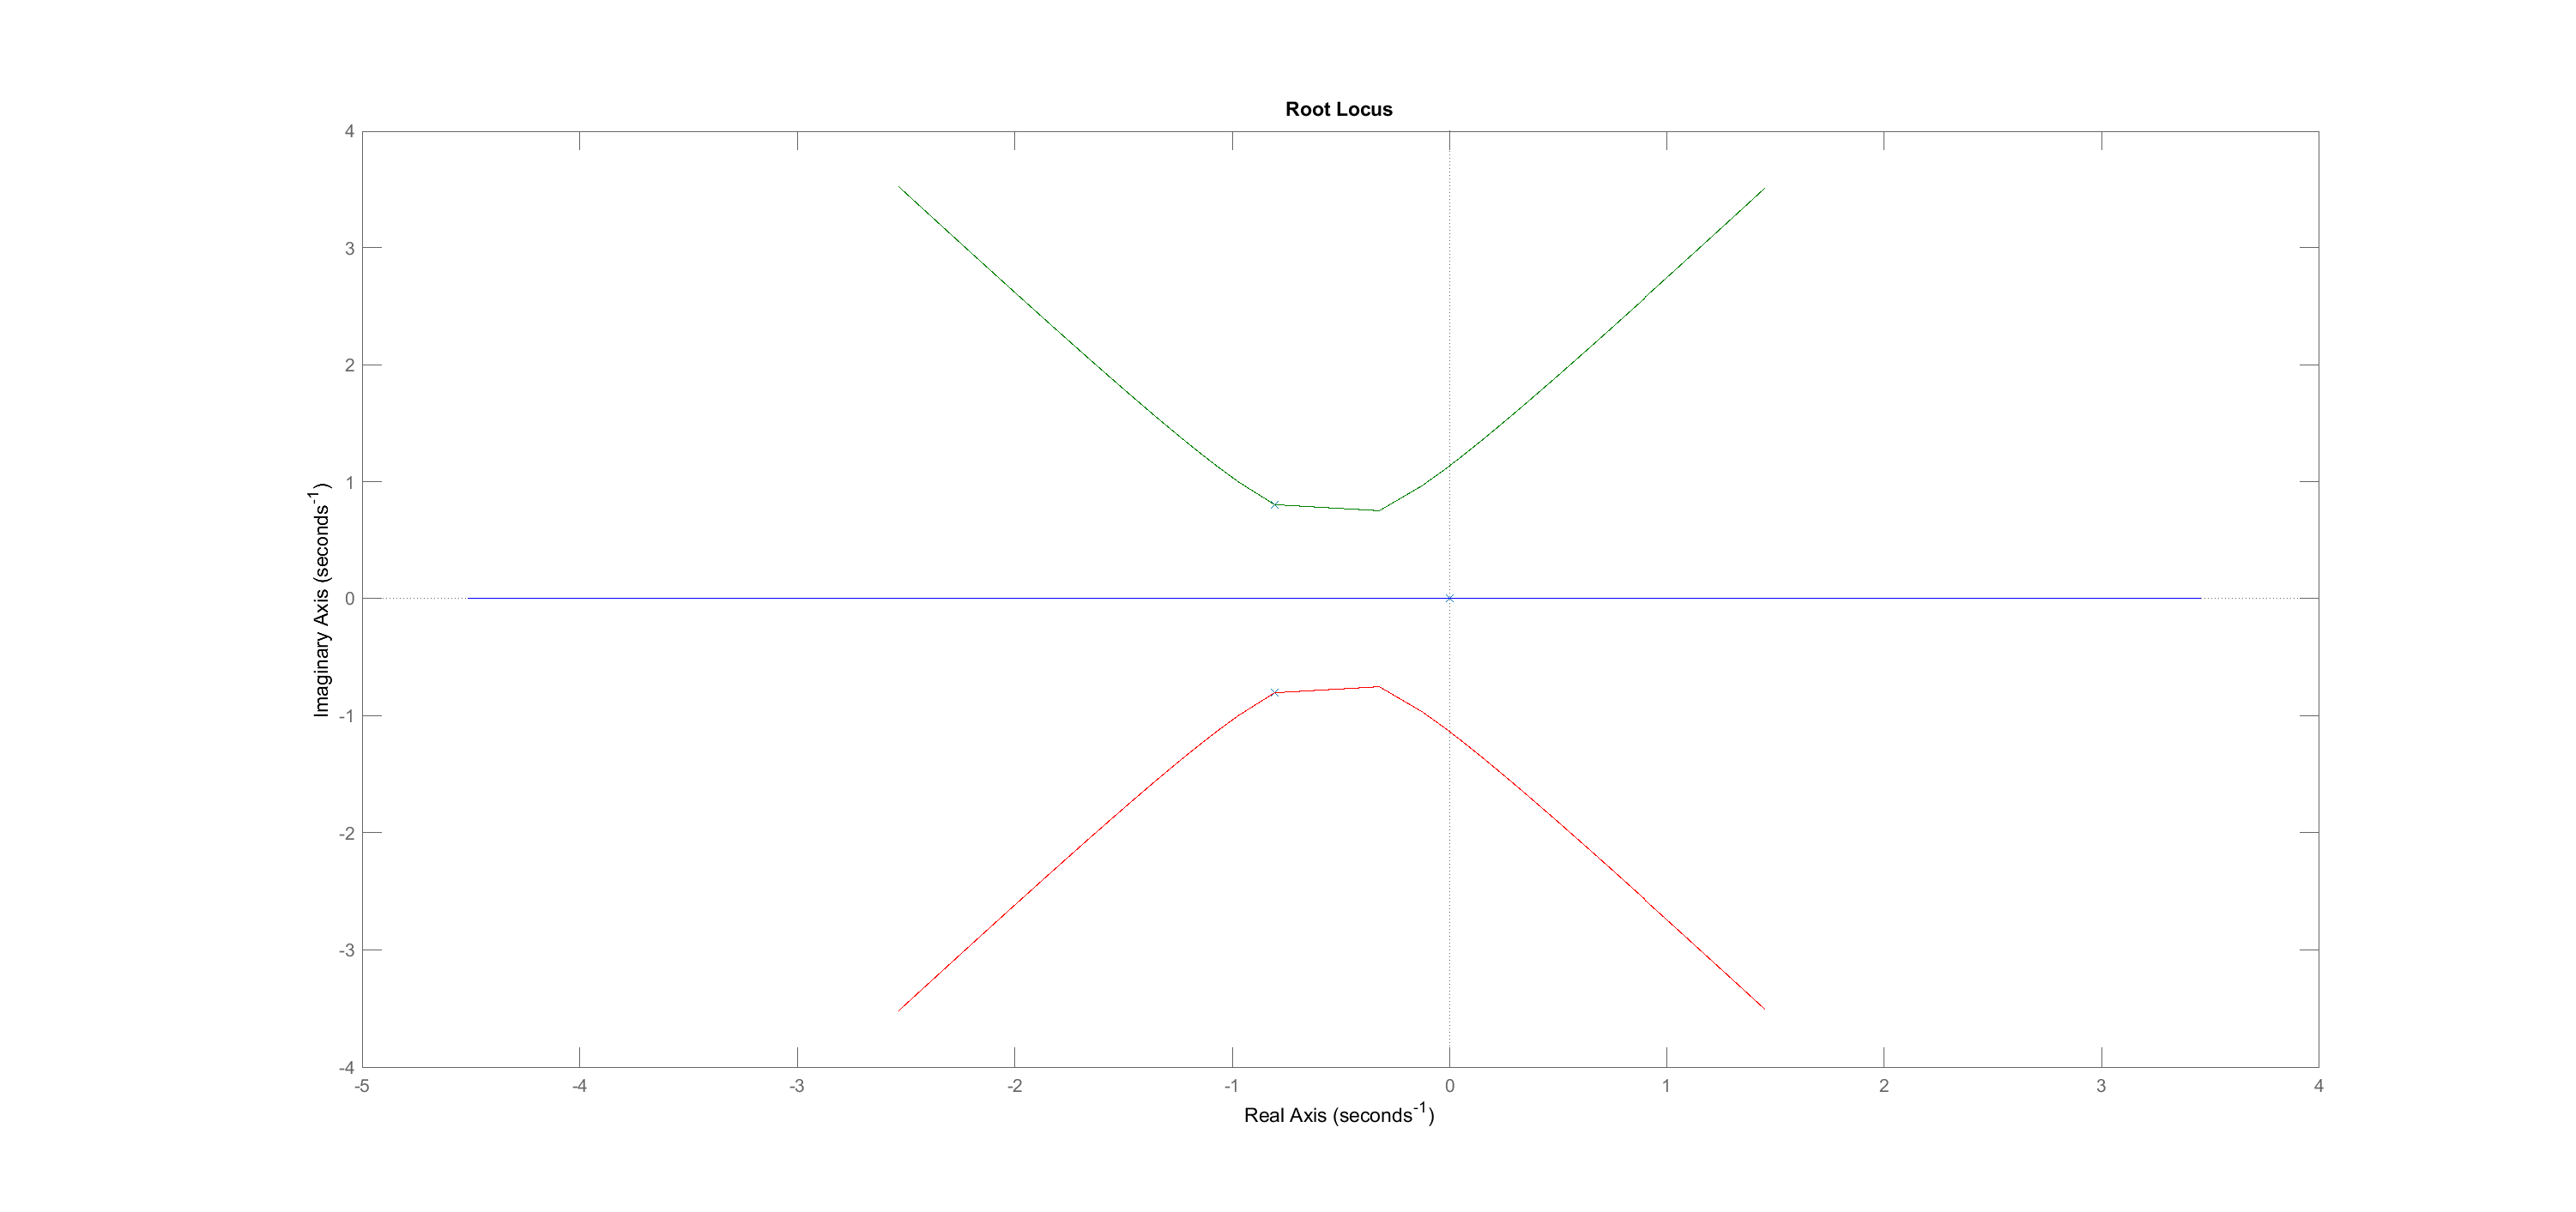
\includegraphics[width=\textwidth]{figures/root_locus_k_i_phi}
		\caption{Root locus with range $k_{i_\phi}$ from -100 to 100}
		\label{fig:root_locus_large_range}
	\end{subfigure}
	\begin{subfigure}[b]{0.45\textwidth}
		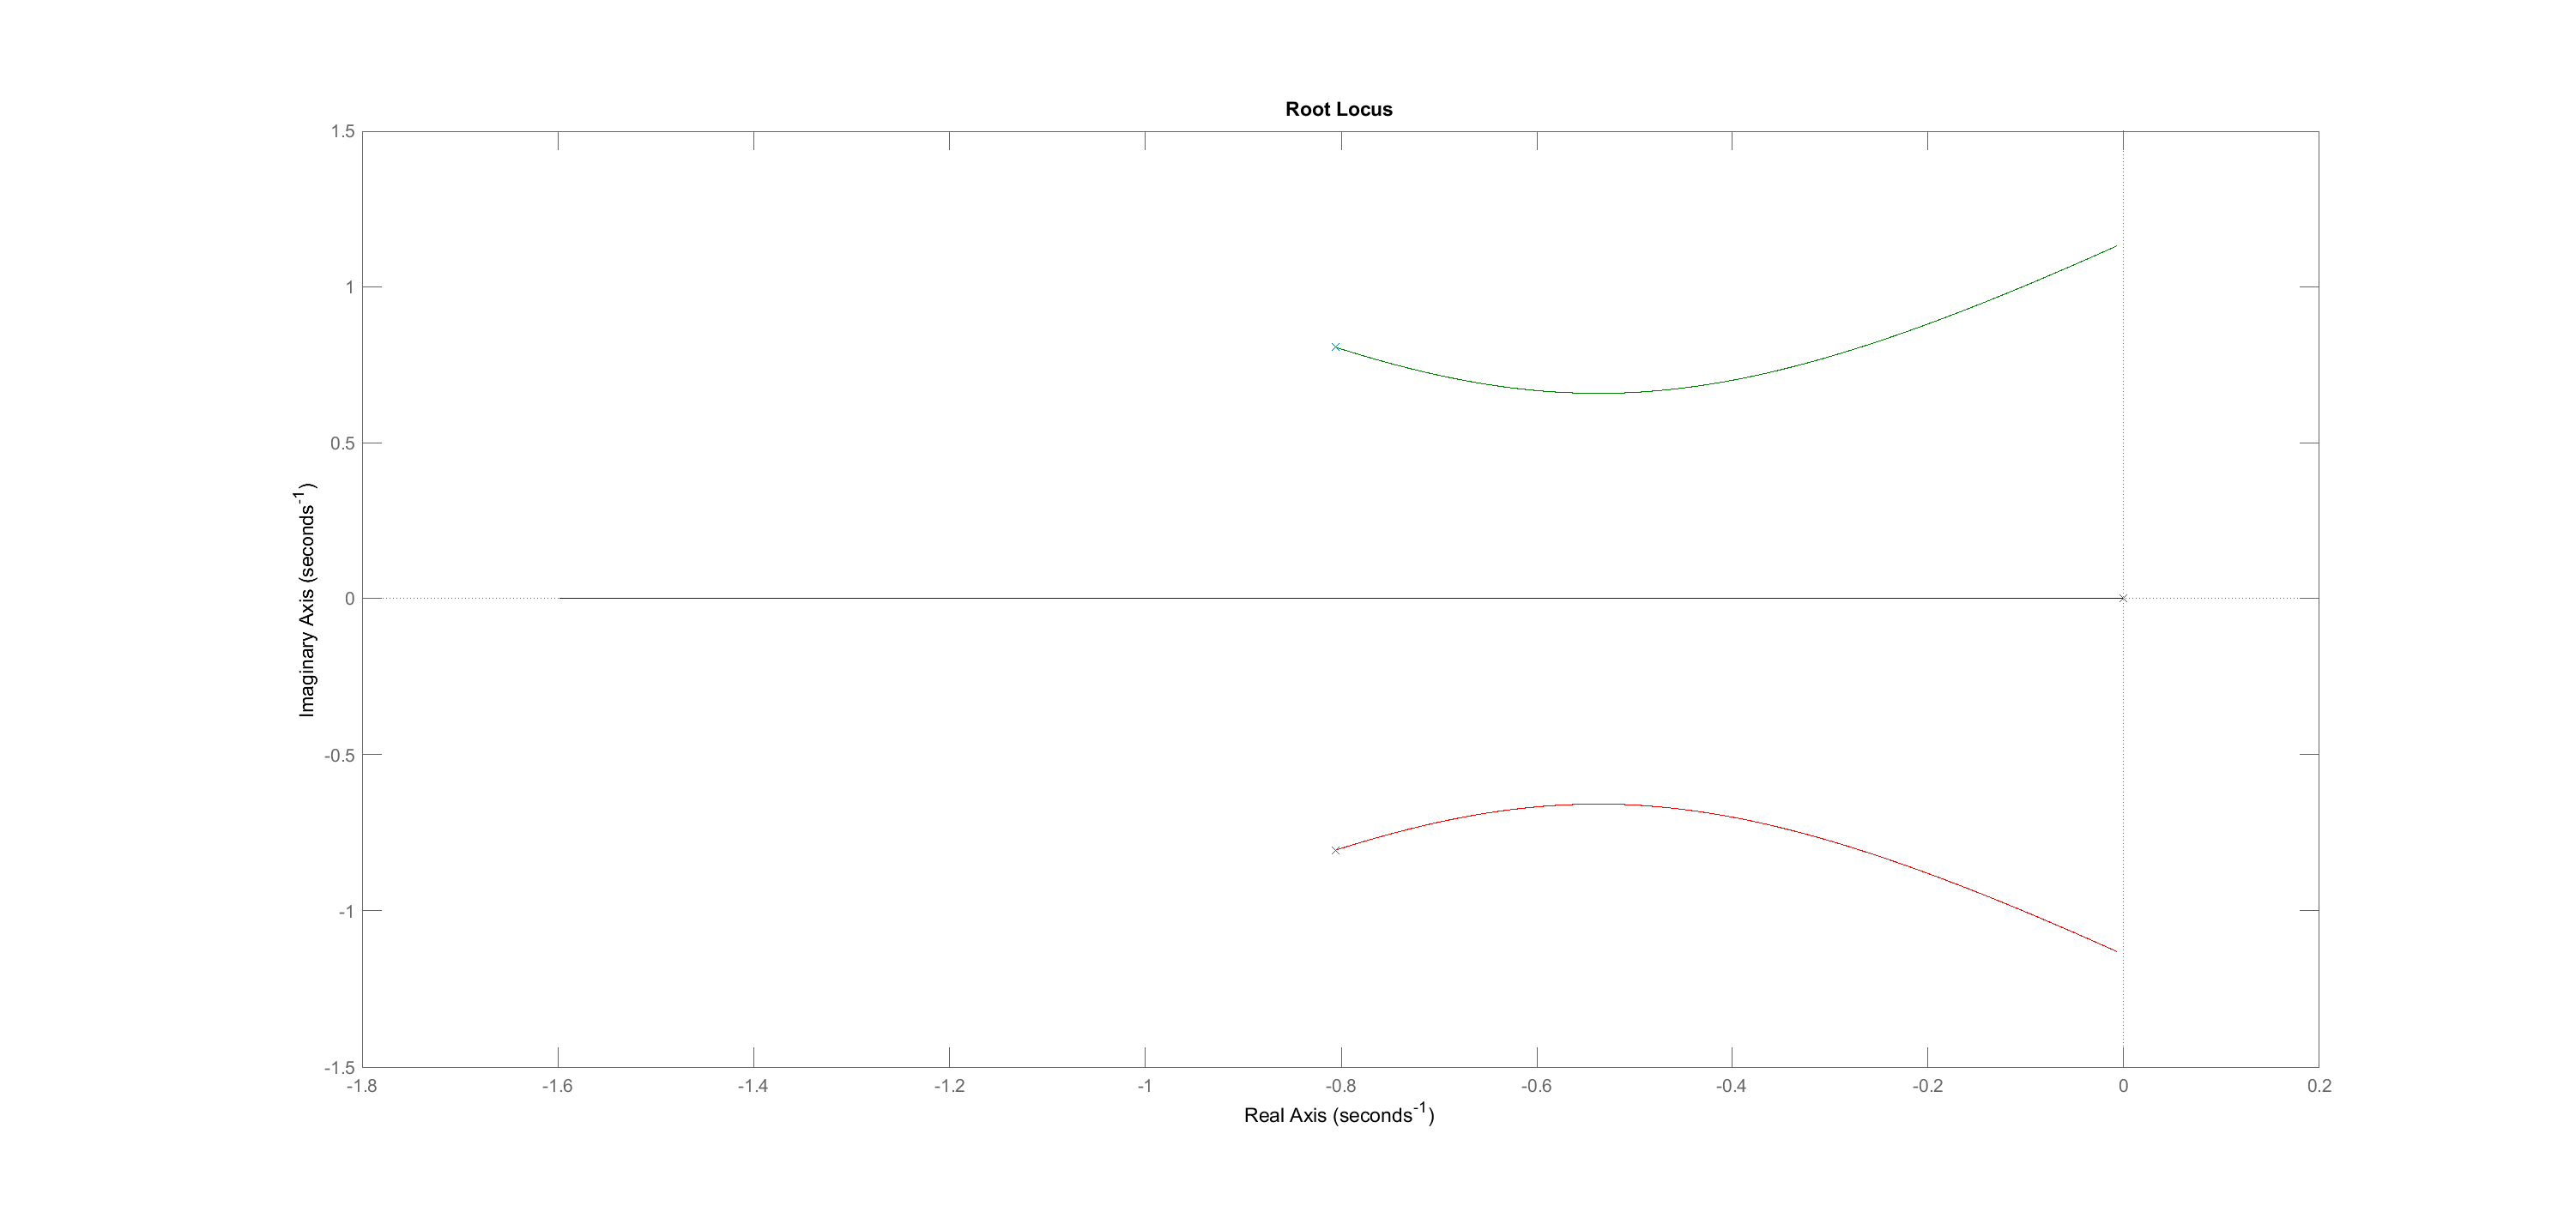
\includegraphics[width=\textwidth]{figures/root_locus_k_i_phi_interval_minus_pi_to_0}
		\caption{Root locus with range $k_{i_\phi}$ from -$\pi$ to 0}
		\label{fig:root_locus_proper_range}
	\end{subfigure}
\end{figure}

From this figure, we can conclude that the range seems to be slightly smaller than $-\pi$, but not by much, so that the range seems to be around $[-3.2, 0]$, but we are using $-\pi$ as it's a more interesting number. 

Further, choosing a lower $\omega_{n_\chi}$ by using $W_\chi = 10$ we may set $\zeta_\chi = 2$ a little higher without issue. Then we can find:
\begin{align*}
    \omega_{n_\chi} &= \frac{1}{W_\chi} \omega_{n_\phi} 
    = \frac{1}{10} 1.140 \approx 0.114 \\
    k_{p_\chi} &= \frac{2 \zeta_\chi \omega_{n_\chi} V_g}{g} 
    = \frac{2 * 2 * 0.114 * 580}{9.81 * 3.6} 
    \approx 7.49 \\
    k_{i_\chi} &= \frac{\omega_{n_\chi}^2 V_g}{g}
    = \frac{0.114^2 * 580}{9.81 * 3.6} 
    \approx 0.214
\end{align*}

\subsection{}
There doesn't seem like there's a need for an integrator for this model. The integrator is usually needed for removing a disturbance that enters before $\delta_a$ in Figure 1 of the assignment task. As there is no disturbance here, the only reason we'd need an integral term would be to stabilize the system, but we can see from the root-locus analysis that the system is stable for $k_{i_\phi} = 0$. Therefore, we may choose this value. 

\subsection{}

\begin{figure}[ht]
	\centering
	\begin{subfigure}[b]{0.45\textwidth}
		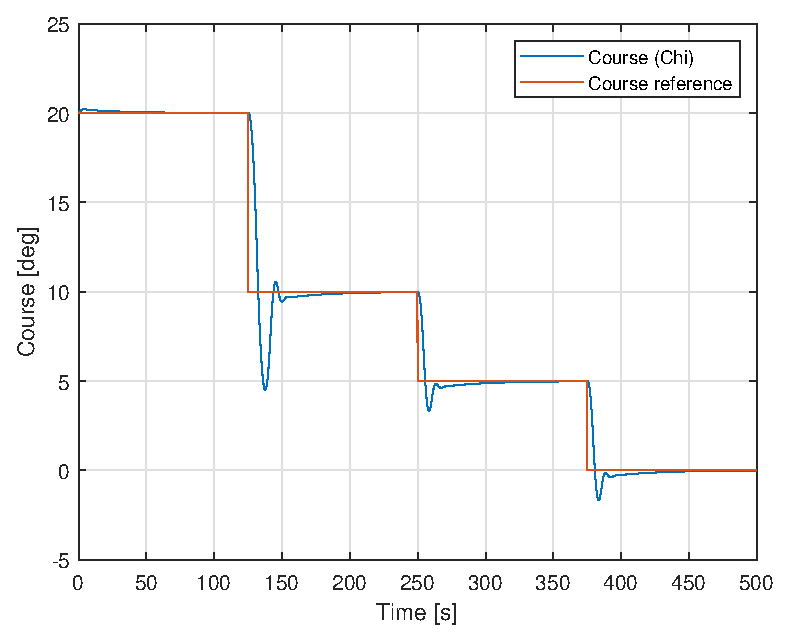
\includegraphics[width=\textwidth]{figures/2d_chi_course}
		\caption{The course and course reference $\chi$}
		\label{fig:2d_chi_course}
	\end{subfigure}
	\begin{subfigure}[b]{0.45\textwidth}
		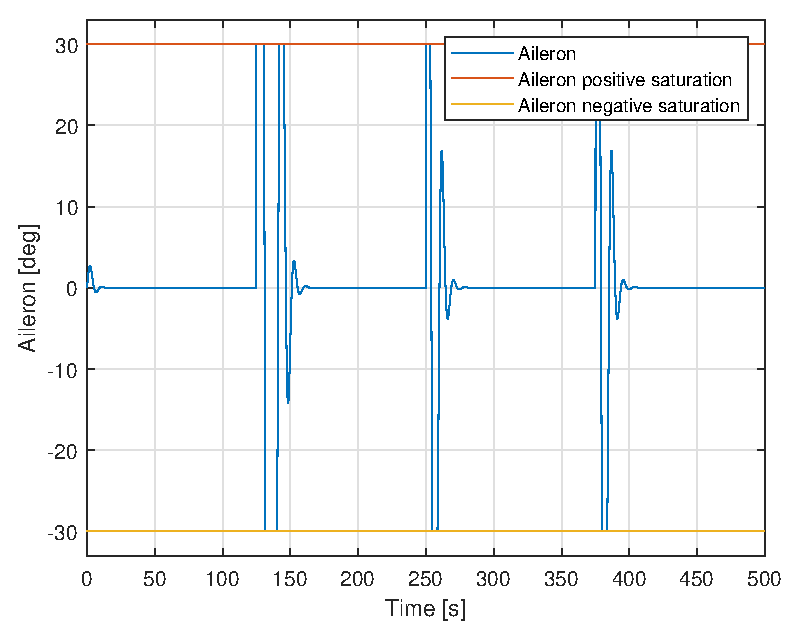
\includegraphics[width=\textwidth]{figures/2d_delta_a_aileron}
		\caption{The aileron with saturation $\delta_a$}
		\label{fig:2d_delta_a_aileron}
	\end{subfigure}
\end{figure}

The results seem good and well controlled, and we can note that the integral term for $\phi$ was unnecessary, as discussed earlier. 

\subsection{}

\begin{figure}[ht]
	\centering
	\begin{subfigure}[b]{0.45\textwidth}
		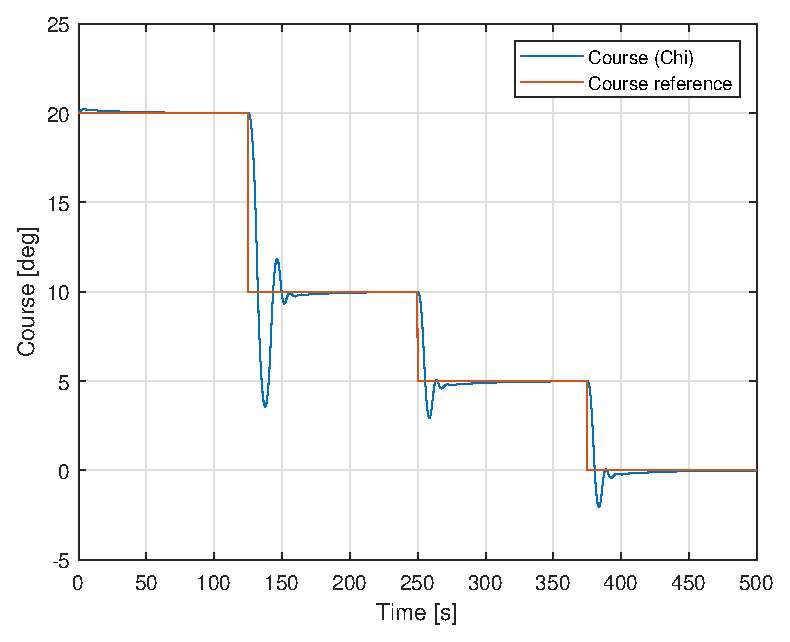
\includegraphics[width=\textwidth]{figures/2e_chi_course}
		\caption{The course and course reference $\chi$}
		\label{fig:2e_chi_course}
	\end{subfigure}
	\begin{subfigure}[b]{0.45\textwidth}
		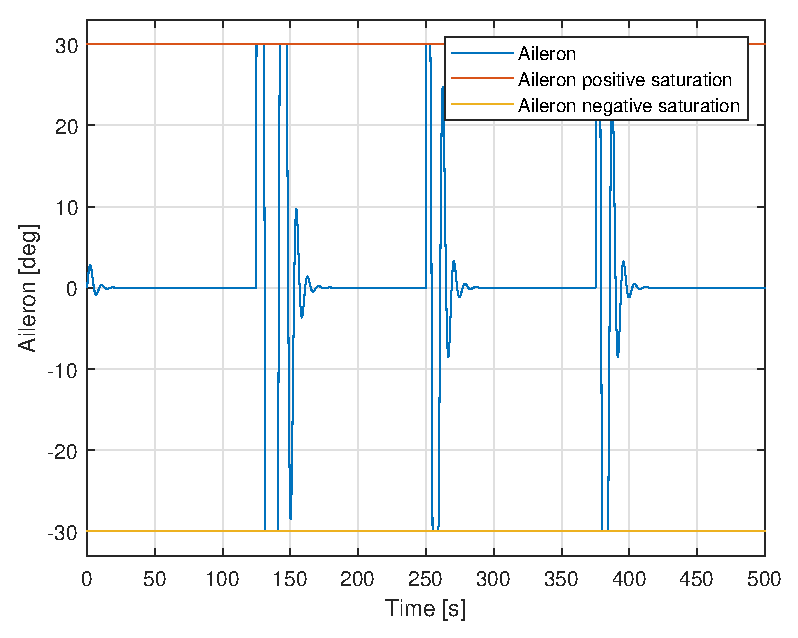
\includegraphics[width=\textwidth]{figures/2e_delta_a_aileron}
		\caption{The aileron with saturation $\delta_a$}
		\label{fig:2e_delta_a_aileron}
	\end{subfigure}
\end{figure}

As we can see when comparing the figures, especially the courses \figref{fig:2d_chi_course} and \figref{fig:2e_chi_course}, the simplified model reproduces the true dynamics very well. The system is still stable, and the values still converge quite quickly towards the reference points. 

\subsection{}
Integrator windup doesn't seem like a big problem in these simulations, though we can see the overshoot in \figref{fig:2e_chi_course} and \figref{fig:2d_chi_course}. This is due to the integrator windup. This is caused by a large error over time causing the input to saturate. 

One method for handling this could be to turn the integrator off while the input is saturated. Thereby the integrator will not integrate up any error due to saturation. Another method could be to have a certain cutoff value for the integrator. Using this we may reset (set to zero) any integrator which are too large. 

Another method still would be to calculate both the saturated and unsaturated inputs, and then incrementing the integrator by a proportion of the input difference: 

\begin{align*}
	\Delta I = \frac{1}{k_i} (u - u_{\text{unsat}})
\end{align*}

This will end up subtracting the exact amount needed so that the input can be kept at the saturation point, rather than keep increasing the longer the input is saturated. 

Implementing the first method (not increasing the integrator while saturated), we can see the results in \figref{fig:2f_chi_course} and \figref{fig:2f_delta_a_aileron}. This is not exactly the results we'd expect, as the integrator still seems to jump whenever there's a saturation. We've further tested the other methods, but we still get a slight \textit{dip} in \figref{fig:2f_chi_course}.

\begin{figure}[ht]
	\centering
	\begin{subfigure}[b]{0.45\textwidth}
		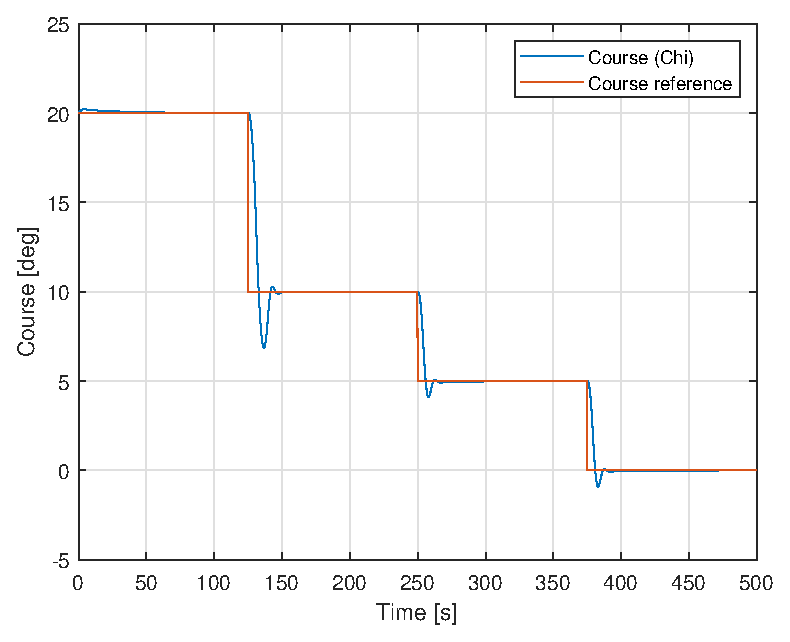
\includegraphics[width=\textwidth]{figures/2f_chi_course}
		\caption{The course and course reference $\chi$}
		\label{fig:2f_chi_course}
	\end{subfigure}
	\begin{subfigure}[b]{0.45\textwidth}
		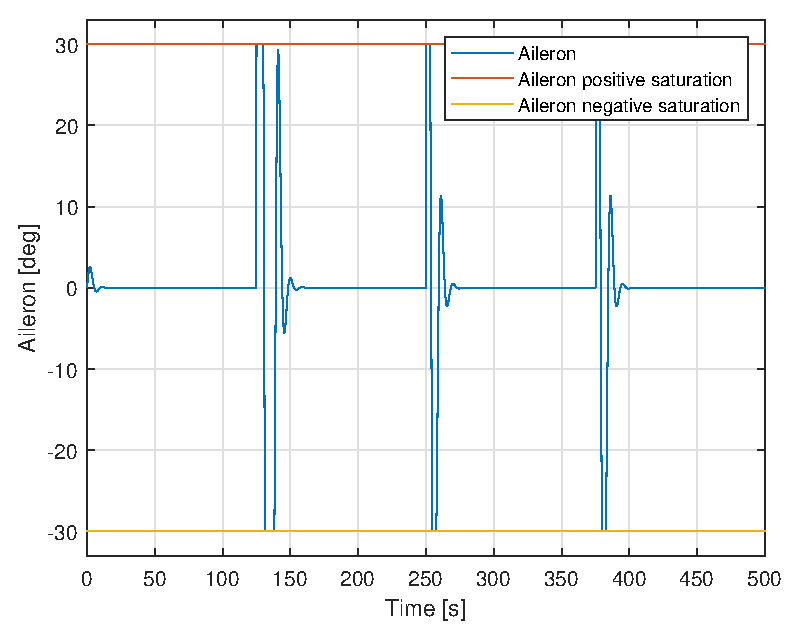
\includegraphics[width=\textwidth]{figures/2f_delta_a_aileron}
		\caption{The aileron with saturation $\delta_a$}
		\label{fig:2f_delta_a_aileron}
	\end{subfigure}
\end{figure}

\bibliographystyle{IEEEtran}
\bibliography{bibliography.bib}

\end{document}
